\section{Object recognition by BOW}

\subsection{Classification and feedback}

{\bfseries (a) Add a function to visualize the images in a green framework if the classification is correct and in a red framework if it does not}

The source code to conduct this task is located at \texttt{ex1.m} and \texttt{classify\_and\_show.m}. Basically what we do is to read the \texttt{tiny-model.mat} file generated by the script \texttt{phow\_caltech101.m} which, among other things contain the SVM's weights and offsets to classify the images. We believe that the code is straightforward enough, so we refer the reader to the annex and to the scripts themselves to see more details. We can see some results in figure \ref{fig:examples-of-image-classification}.

\begin{figure}[htb]
	\centering
	\begin{subfigure}[t]{0.4\textwidth}
		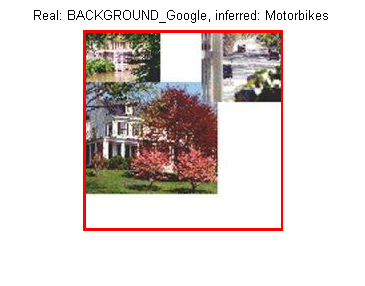
\includegraphics[width=\textwidth]{./img/ex1/bg_google.png}
		\caption{\emph{BACKGROUND\_google} image incorrectly classified as \emph{Motorbike}}
	\end{subfigure}
	
	\begin{subfigure}[t]{0.4\textwidth}
		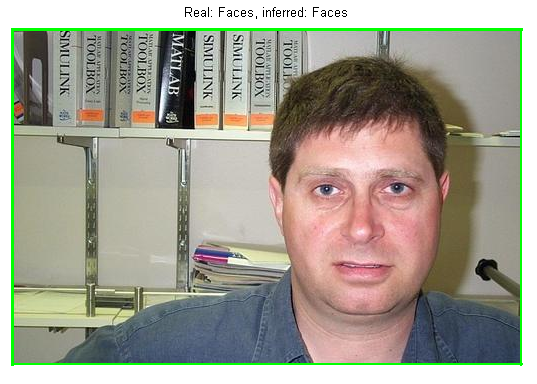
\includegraphics[width=\textwidth]{./img/ex1/faces.png}
		\caption{\emph{Faces} image correctly classified}
	\end{subfigure}
	~
	\begin{subfigure}[t]{0.4\textwidth}
		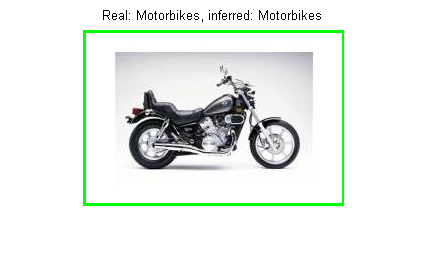
\includegraphics[width=\textwidth]{./img/ex1/motorbike.png}
		\caption{\emph{Motorbike} image correctly classified}
	\end{subfigure}
	
\caption{Examples of image classification}
\label{fig:examples-of-image-classification}
\end{figure}

\subsection{PHOW descriptors}

{\bfseries (b) What are the PHOW descriptors? What does the Sizes parameter mean? What does happen if the Sizes parameter is augmented? What does the Step parameter mean? What does happen if the Step parameter is augmented?}

PHOW stands for Pyramid Histogram Of visual Words. The PHOW descriptors are those of SIFT, only that obtained with the dense variant of the algorithm. In this variation several points are evaluated in a reduced number of scales. In our particular case (\emph{tiny} problem) we use one scale. The scale(s) is specified with the \emph{Sizes} parameter. The \emph{Sizes} parameter is initially set to 7. Should the \emph{Sizes} parameter be increased, PHOW will extract features that correspond to high scale image structures.  We can appreciate the effect of incrementing the scale from 7 to 14 in figure \ref{fig:effect-size-accuracy}. We can observe that the accuracy actually improves. This let us to believe that the most adequate value for the \emph{Size} is the one that adapts to the structures that best discriminate between images of different categories. Another consequence of changing this parameter is a significant reduction of the (vocabulary) training time, as shown in table \ref{fig:effect-size-time}. Therefore, in this particular case it would seem that setting \emph{Sizes} to 14 is a win-win situation.

\begin{figure}[htb]
	\centering
	\begin{subfigure}[t]{0.4\textwidth}
		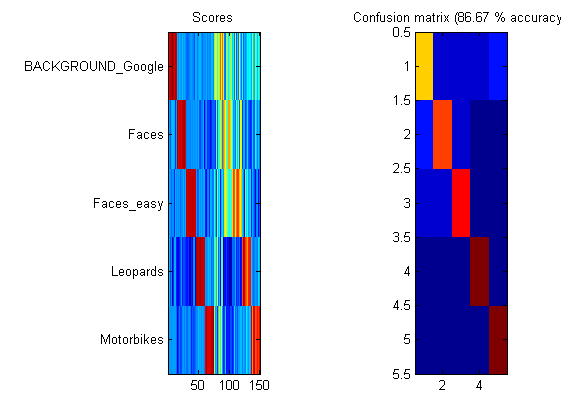
\includegraphics[width=\textwidth]{./img/ex1/eval-initial.png}
		\caption{Initial results (Size=7, Steps=5)}
	\end{subfigure}
	~
	\begin{subfigure}[t]{0.4\textwidth}
		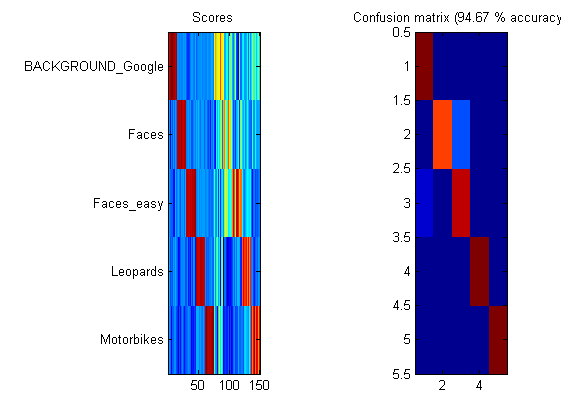
\includegraphics[width=\textwidth]{./img/ex1/eval-size-14.png}
		\caption{$ Size=14 $}
	\end{subfigure}
	
\caption{Effect in terms of accuracy of increasing \emph{Size} from 7 to 14}
\label{fig:effect-size-accuracy}
\end{figure}

\begin{table}[htb]
	\centering
	\begin{tabular}{l|rr}
		{\bfseries Elapsed time} 			 & {\bfseries Training vocabulary} & {\bfseries Testing} \\ \hline
		{\bfseries Initial parameters} & 142.73s												 & 0.57s \\
		{\bfseries Sizes=14}           & 122.21s												 & 0.56s \\
	\end{tabular}
	\caption{Effect in terms of time of increasing \emph{Size} from 7 to 14}
	\label{fig:effect-size-time}
\end{table}

In dense SIFT the key points are chosen from a reduced number of candidate distributed in a grid fashion. The evaluated pixels are separated from each other by a fixed distance, which is the \emph{Step} parameter. In our case, the \emph{Step} is initially set to 5. If we set the \emph{Step} parameter to a higher value, the training (actually the extraction of the vocabulary which is more of a preprocessing step) and the predictions will be significantly faster, but there will fewer candidate pixels for choosing the key points (and therefore, a reduced number of descriptors). We see the effects in terms of accuracy of increasing the \emph{Step} from 5 to 10 and to 20 in figure \ref{fig:effect-steps-accuracy}. The accuracy does not get worse until we set the step as high as 20. In addition it is possible to appreciate the notable speedup in the training phase in table \ref{tab:effect-steps-time}.

\begin{figure}[htb]
	\centering
	\begin{subfigure}[t]{0.4\textwidth}
		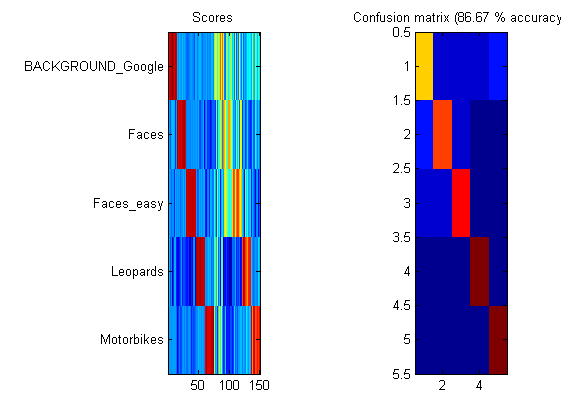
\includegraphics[width=\textwidth]{./img/ex1/eval-initial.png}
		\caption{Initial results (Size=7, Steps=5). Acc: 86.67\%}
	\end{subfigure}
	
	\begin{subfigure}[t]{0.4\textwidth}
		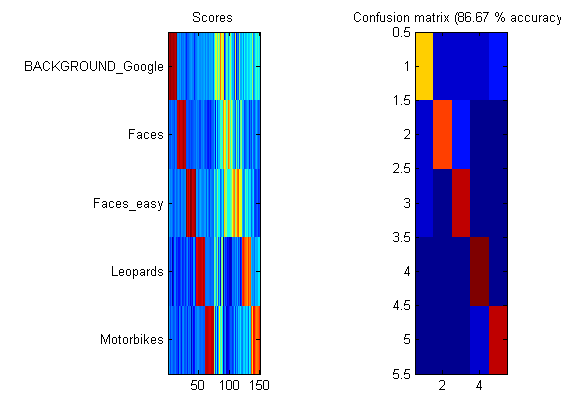
\includegraphics[width=\textwidth]{./img/ex1/eval-steps-10.png}
		\caption{$ Steps=10 $. Acc: 86.67\%}
	\end{subfigure}
	~
	\begin{subfigure}[t]{0.4\textwidth}
		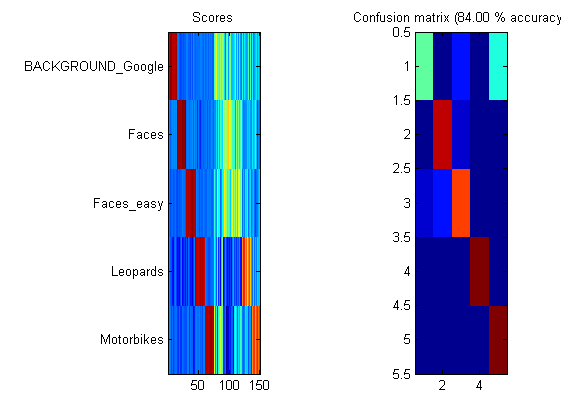
\includegraphics[width=\textwidth]{./img/ex1/eval-steps-20.png}
		\caption{$ Steps=20 $. Acc: 84\%}
	\end{subfigure}
\caption{Effect in terms of accuracy of increasing \emph{Step}}
\label{fig:effect-steps-accuracy}
\end{figure}

\begin{table}[htb]
	\centering
	\begin{tabular}{l|rr}
		{\bfseries Elapsed time} 			 & {\bfseries Training vocabulary} & {\bfseries Testing} \\ \hline
		{\bfseries Initial parameters} & 142.73s												 & 0.57s \\
		{\bfseries Step=10}            & 19.07s												   & 0.45s \\
		{\bfseries Step=20}            & 4.00s												   & 0.45s \\
	\end{tabular}
	\caption{Effect in terms of time of increasing \emph{Step}}
	\label{tab:effect-steps-time}
\end{table}

\subsection{Extraction of the vocabulary}

{\bfseries (c) What are the words in the algorithm? How are they extracted? What is their dimension? How their number does affect the accuracy of the results?}

The words consist in SIFT descriptors. However, these descriptors are not directly the descriptors extracted from the images. An unsupervised learning procedure receives these descriptors and obtains a set of clusters that summarizes them all. More specifically, the algorithm uses K-means with the Elkan heuristic for reducing the computing effort. The centroids of the obtained clusters are used as the vocabulary words.

Since the words are just SIFT descriptors, their dimension is 128. The effect of the number of words can be understood in terms of the concepts of overfitting and underfitting. Too few and they will not be able to capture all the particular structures that can help in the discrimination between two images (underfitting or high bias). Too many and they will be too specific for the images in the training set (overfitting or high bias).

{\bfseries (d) To construct the vocabulary, the method uses the k-means algorithm. Explore and explain how the k-means is applied, which parameters are used, what is there meaning and what are the advantages and the limitations of the method.}

As said before, the k-means algorithm is applied to the descriptors extracted from the images of the train set. The most important parameter (after the descriptors, of course) is the number of desired clusters which is, of course, the number of works we want in our vocabulary. The computational effort of the vanilla K-means is counteracted with the Elkan heuristic that avoids the computation of several distances by application of the triangular inequality. The main drawback of this is that uses storage proportional to the number of clusters\footnote{\url{http://www.vlfeat.org/api/kmeans-fundamentals.html}}, so it is not advisable for problems in which we want a high amount of clusters. The use of this heuristic (or any other) is specified as a parameter. Another problem with K-means is that it cannot adapt to clusters with arbitrary forms. An alternative that provides some flexibility in this regard is the well-known EM (Expectation-Maximization) algorithm, which assumes Gaussian clusters with arbitrary covariance matrices. However, this algorithm is more computational intensive and we have already seen that the use of K-means already leads to good results.

\subsection{Spatial histograms: the image descriptor}

{\bfseries (e) The function getImageDescriptor gives the spatial histogram of the image. What is the spatial histogram? What dimension does it have? What happens if we augment model.numSpatialX from 2 to 4?}

In order to include some knowledge about the location of the visual words in the image, it is divided into smaller quadrants. Initially, the image is divided into $ 2 \times 2 $ sectors, as per the \emph{numSpatialX} and the \emph{numSpatialY} parameters. Instead of counting the number of word occurrences in the whole image, we count the number of words in each sector. Therefore, the image descriptor consists of the count of word occurrences for each quadrant. In other words, the total dimension of the image descriptor (which is not the same as the PHOW descriptors) is the number of words times the number of quadrants. This is the spatial histogram and it is what is computed by the \emph{getImageDescriptor} method.

Should we increment \emph{numSpatialX} (or for that matter \emph{numSpatialY}) from 2 to 4, we would multiply by 2 the number of sectors and, consequently, the dimension of the spatial image histogram.

In figure \ref{fig:effect-size-numSpatialX} we can see that setting \emph{numSpatialX} to 4 has led to a slight increase in the accuracy.

\begin{figure}[htb]
	\centering
	\begin{subfigure}[t]{0.4\textwidth}
		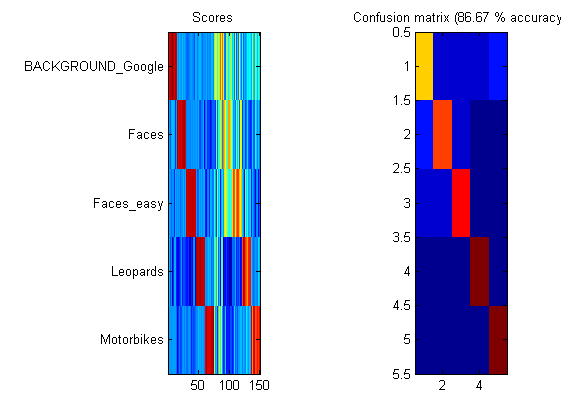
\includegraphics[width=\textwidth]{./img/ex1/eval-initial.png}
		\caption{Initial results (numSpatialX=2)}
	\end{subfigure}
	~
	\begin{subfigure}[t]{0.4\textwidth}
		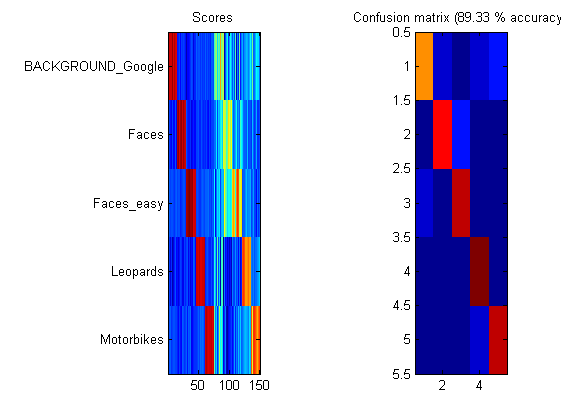
\includegraphics[width=\textwidth]{./img/ex1/eval-numSpatialX-4.png}
		\caption{$ numSpatialX=4 $}
	\end{subfigure}
	
\caption{Effect in terms of accuracy of increasing numSpatialX from 2 to 4}
\label{fig:effect-size-numSpatialX}
\end{figure}

\subsection{SVM classification}

{\bfseries (f) The SVM classification with homogeneous kernels is performed by the vl\_svmtrain function that needs the homogeneous kernel map obtained by the vl\_homkermap function. What are the parameters obtained after the training process? What dimension do they have? How do you apply them to obtain the score of the final classification?}

The parameters obtained after the training process are the weight vector (the \emph{w}) and the offset (the \emph{b}). The score is obtained performing the inner product between the weights vector and the input transformed by the homogeneous kernel map (the \emph{psix} vector) and adding to that the offset. This is done with a different \emph{w} and \emph{b} for each of the classes since we are performing a One vs All classification.

The input data is the spatial histogram, which has a dimension of 1200 ($ 300 \mathrm{words} \times 4 \mathrm{sectors} $). However the transform maps the data into a higher dimensional space. The \emph{psix} vector has a dimension of 3600. The dimensions of the weight vector \emph{w} are consistent with this (i.e. also a vector with 3600 rows). Since we are working with 5 classes, we have 5 columns for \emph{w} and 5 for \emph{b}.

\subsection{Robustness against image transformations}

{\bfseries (g) Is the algorithm invariant to rotation of the images? Is the algorithm invariant to rescaling of the images?}

If by \emph{rotation of the images} we understand rotation both of the training images and of the test images (or in general any other image that is classified after training the SVM), then sure enough the algorithm will be invariant to rotation (after all this is one of the strengths of the SIFT algorithm that is used to extract the descriptors). On the other hand, if we mean that the test images that are later passed to the classifier are rotated with respect to what the classifier expects, then the classification will fail due the fact that we are using spatial histograms. As long as there are more than one sector (i.e. $ numSpatialX > 1 \lor numSpatialY > 1 $) the algorithm will be prone to fail in the presence of strong rotations (e.g. a car upside down when the classifier was training with cars normally orientated).

On the other the algorithm is invariant to the rescale of the image (or almost, after all we cannot expect it to work if we scale the image down to one pixel). Again the SIFT descriptors provide us this robustness. In fact, it is worth mentioning that before extracting the spatial histogram, the algorithm scales the image so it has a fixed height of 480.

\subsection{On the effect of increasing the number of classes}

{\bfseries (h) Compute how the accuracy changes when the number of categories augment (e.g. from 5 to 10 to 15 to 100).}

\textbf{NOTE:} in order to perform this check faster, we have set the \emph{Step} parameter to 10. While it does not alter the accuracy when using 5 classes it can affect the results with a higher number of classes. Even so, we believe that the results are still orientative.

As one could anticipate, increasing the number of classes affects negatively the performance of the classifier. The greater the number of classes it has to identify, the more prone it will be to failure. Figure \ref{fig:effect-classes} illustrates this issue.

\begin{figure}[htb]
	\centering
	\begin{subfigure}[t]{0.4\textwidth}
		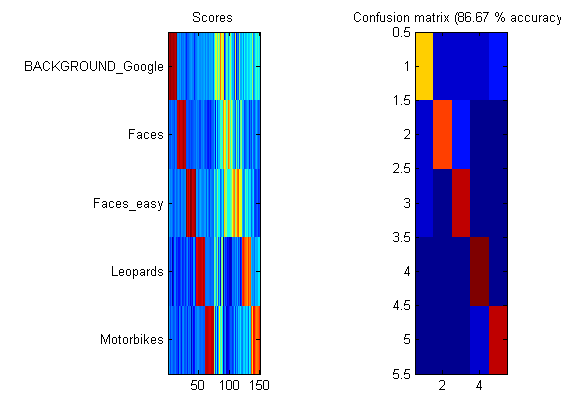
\includegraphics[width=\textwidth]{./img/ex1/eval-steps-10.png}
		\caption{Results with 5 classes (Acc 86.67\%)}
	\end{subfigure}
	~
	\begin{subfigure}[t]{0.4\textwidth}
		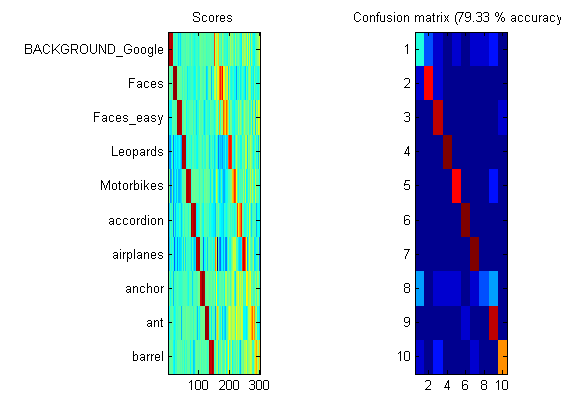
\includegraphics[width=\textwidth]{./img/ex1/eval-10-classes.png}
		\caption{Results with 10 classes (Acc 79.33\%)}
	\end{subfigure}
	
	\begin{subfigure}[t]{0.4\textwidth}
		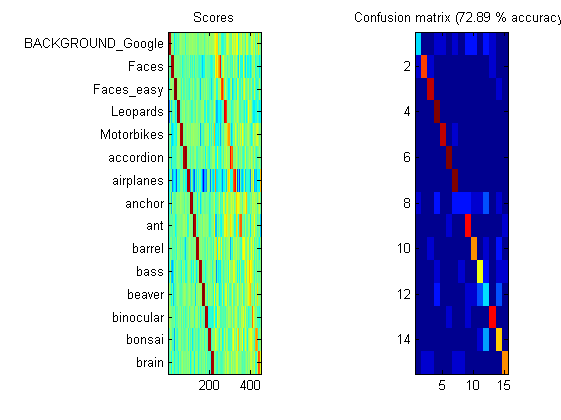
\includegraphics[width=\textwidth]{./img/ex1/eval-15-classes.png}
		\caption{Results with 15 classes (Acc 72.89\%)}
	\end{subfigure}
	~
	\begin{subfigure}[t]{0.4\textwidth}
		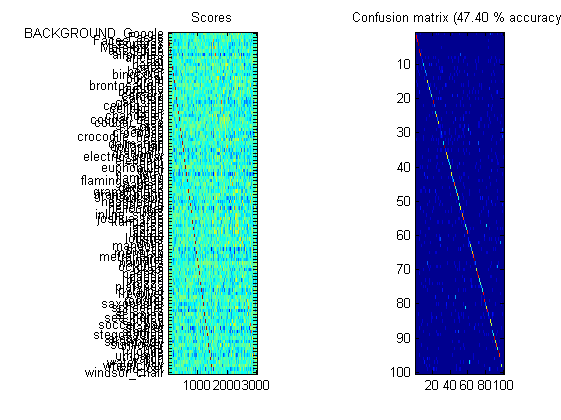
\includegraphics[width=\textwidth]{./img/ex1/eval-100-classes.png}
		\caption{Results with 100 classes (Acc 47.40\%)}
	\end{subfigure}
\caption{Effect of increasing the number of classes}
\label{fig:effect-classes}
\end{figure}

The accuracy in problems for large number of classes has to be optimized by means of tweaking the different parameters that govern the algorithm. For instance, for a larger number of classes one could think that extending the vocabulary, increasing the number of sectors or adding more scales to the PHOW feature extractor is a good idea. This is not covered in the present document.